%%%%%%%%%%%%%%%%%%%%%%%%%%%%%%%%%%%%%%%%%%%%%%%%%%%%%%%%%%%%%%%%%%%%%%%%%%%%%%%
% CAPÍTULO 3 - GESTIÓN DE CÓDIGO Y PROCESO DE DESARROLLO
%%%%%%%%%%%%%%%%%%%%%%%%%%%%%%%%%%%%%%%%%%%%%%%%%%%%%%%%%%%%%%%%%%%%%%%%%%%%%%%
\chapter{Gestión de código y proceso de desarrollo}
\label{chap:codeManagement}
\begin{comment}
Introducción de lo que es el proyecto, lo del libro de Python y luego las tecnologías usadas en el proyecto unidas con la introducción.
\end{comment}
En este capítulo trataremos como está compuesto el proyecto y como se ha gestionado este, tanto la parte del código fuente de nuestro paquete \emph{PyCardio} como el código que forma parte de nuestro proyecto web. En dicho proyecto se presenta la documentación de PyCardio, incluyendo manuales de usuario y una descripción de sus funcionalidades principales. \\
Para ello dividiremos el capítulo en tres secciones:
\begin{enumerate}
    \item Explicación de que contiene el proyecto \emph{PyCardio} mediante un breve resumen de los módulos que la componen. 
    \item Buenas prácticas de desarrollo en Python y como escribir buen código.
    \item Identificación de los elementos de nuestro proyecto con las tecnologías descritas en el capítulo \ref{chap:Arqui}, para la gestión de proyecto del Backend.
\end{enumerate}

        %%%%%%%%%%%%%%%%%%%%%%%%%%%%%%%%%
        %% EXPLICACIÓN DE CONTENIDO
        %%%%%%%%%%%%%%%%%%%%%%%%%%%%%%%%%
\section{¿Que és PyCardio?}
\label{sec:explainPyCardio}
\emph{PyCardio} es un módulo en desarrollo  de Python creado por varios profesores del Grupo de Teoría de la Señal y Comunicaciones de la ETSIT, en la URJC. Dicho módulo tiene el objetivo de realizar análisis de las señales cardíacas. Los tipos de análisis actualmente incluidos en la herramienta son:
\begin{itemize}
    \item \textbf{ECG Análisis}: Detección del complejo QRS, extracción de series temporales de intervalo RR, delineación completa de ECG.
    \item \textbf{Análisis de variabilidad de la frecuencia cardíaca}: Un análisis completo de las series temporales de intervalo RR, donde se realiza un preprocesado, análisis en  el dominio del tiempo, análisis en el dominio de la frecuencia, análisis no lineal y un análisis tiempo-frecuencia.
    \item \textbf{Análisis de la frecuencia cardiaca de turbulencia.}
    \item \textbf{Análisis de fibrilación auricular.}
    \item \textbf{Análisis de fibrilación ventricular.}
    \item \textbf{Análisis de arritmia mediante un dispositivo de monitorización portátil.}
\end{itemize}

El objetivo, por tanto, es la creación de una página web que muestre estas funcionalidades, así como una guía de instalación, documentación, y una orientación de como colaborar en el proyecto mediante las tecnologías mencionadas en el capítulo \ref{chap:Arqui}.

    %%%%%%%%%%%%%%%%%%%%%%%%%%%%%%%%%%%%%%%
    %% BUENAS PRÁCTICAS DE DESARROLLO
    %%%%%%%%%%%%%%%%%%%%%%%%%%%%%%%%%%%%%%
\section{Buenas prácticas de desarrollo en Python}
\label{subsec:bestPracticses}
En esta sección tratamos de explicar y mostrar buenas prácticas para el desarrollo de proyectos en Python. Para ello basaremos todas estas prácticas en una lectura que se ha realizado sobre el libro \emph{The Hitchhiker’s Guide to Python!}\cite{pythonGuide}.\\

\subsection*{Estilo de código}
\label{subsec:stylePython}
Para los \emph{pythonistas} (desarrolladores veteranos de Python) el código fuente de un proyecto es mas leído que escrito, por tanto, el corazón de un proyecto Python es la legibilidad. Una de las razones por las que el código Python es legible es por sus amplias guías de estilo (recogidas en PEP 8 y PEP 20). La comunidad Python intenta hacer lo posible para que sus proyectos se ajusten a estas guías. Tomando como ejemplo uno de los módulos que disponemos en \emph{PyCardio}, podemos ver cuanto sigue nuestro código en el anexo \ref{code:pep8} las reglas de la guía PEP8. \\ 

Estas guías de código suelen integrarse en IDE para facilitarnos su seguimiento,o ejecutar el programa \texttt{autopep8}, que regenera el código siguiendo la guía PEP8. Antes de continuar con las buenas prácticas, no podemos pasar por alto en que consiste PEP y cúal es su propósito. \\
\subsubsection*{¿Qué es PEP?}
PEP son las siglas de Proposal Enhancement Python, son documentos de diseño que proporcionan información de nuevas características del lenguaje Python, de sus procesos o adopción de nuevas reglas. Existen tres tipos de PEP:
\begin{itemize}
    \item PEP estándar: Describe una nueva funcionalidad o característica para Python. 
    \item PEP informativo: En ellos se describen problemas de diseño, pautas a seguir o información para la comunidad.
    \item PEP de proceso: en el se describe procesos que rodean al lenguaje Python o se proponen cambios. Estos cambios que se proponen no son implementaciones al lenguaje base de Python, esos cambios requieren un consenso de la comunidad. 
\end{itemize}

\subsection*{Estructurando el proyecto}
\label{subsec:structurePython}
Por una \emph{estructura} de proyecto de programación nos referimos a como la lógica y las dependencias del código están implementadas. \\
Por tanto seguir una buena estructura de empaquetado y de importación de los módulos que se utilicen en el proyecto proporcionará un código menos repetitivo y desordenado. No existe una manera óptima de estructurar un proyecto pero basándonos en la estructura que propone la guía consultada, reducimos los siguientes errores:
\begin{itemize}
    \item \textit{Dependencias circulares múltiples y desordenadas:} Ocurre cuando un módulo depende de otro, y este a su vez del mismo inicial. Es decir, \textit{fabrica.py} depende de \textit{trabajadores.py}, que depende de \textit{fabrica.py}.
    \item \textit{Un abuso en el uso de contextos globales:} Ocurre cuando dos clases o módulos que hacen uso de la misma variable global, haciendo así que cualquiera de los dos pueda modificarlo.
    \item \textit{Código Ravioli:} hace referencia a que el código se refactoriza en demasiados trozos.
\end{itemize}


\subsection*{Programación orientada a objetos}
Otra característica que destacar cuando estamos trabajando en un proyecto Python es que es un lenguaje orientado a objetos. \\
Esto puede resultar engañoso ya que a diferencia de Java, no impone este paradigma de programación como principal. Por tanto, no es necesario definir clases para desarrollar un proyecto en Python, pero en algunas ocasiones es necesario mantener un estado o un contexto, es decir, necesitamos variables globales de clase. La recomendación a seguir es cuando nos queramos traer entre manos un código con contexto persistente o estado, debemos usar funciones o procedimientos con contextos implícitos y efectos secundarios \footnote{\textbf{Contexto implícito} refiere a código que necesita acceder a variables globales para su función, mientras que \textbf{efectos secundarios} es cuando una función o procedimiento cambia el valor  o estado de una variable global. } lo mínimo posible, es decir reducir el uso de variables globales para que una determinada función realice su trabajo y evitar que estas se modifiquen continuamente. Uno de los objetivos de desarrollar clases personalizadas es aislar funciones con contexto o efectos secundarios, para ello, se aconseja utilizar cuanto más sea posible la programación funcional, es decir, utilizar funciones puras \footnote{Las \textbf{funciones puras} son aquellas funciones que dada una entrada distinta producen la misma salida.}. Las ventajas de usar la programación funcional  a la hora de desarrollar un proyecto son:
\begin{itemize}
    \item Funciones puras son más sencillas de cambiar o reemplazar si se necesita una optimización.
    \item El uso de funciones puras facilita el desarrollo de tests sobre nuestro proyecto.
    \item El tener funciones puras hace más sencillo la manipulación y decoración de estas.
\end{itemize}
Como ya sabemos, Python es un lenguaje dinámicamente tipado, lo que quiere decir que una misma variable puede tomar un valor, e inmediatamente después puede ser una cadena de texto, o una función. Esta característica del lenguaje también puede considerarse una debilidad del mismo, ya que hace muy difícil trazar código.\\

\subsection*{Pruebas de código}
A la hora de distribuir software de código libre, una de las prácticas que hacen que el software sea más utilizado o que ayude a que se sumen contribuciones al software es la prueba del código. ¿Por qué es una de las prácticas para el desarrollo de un proyecto más importante?. (Las siguientes razones son tanto para el ámbito comercial como para un ámbito práctico de desarrollo). 
\begin{itemize}
    \item Porque hasta que una línea de código no es ejecutada, no se puede saber si esta funciona.
    \item En la mayoría de los casos, el código no se ejecuta de principio a fin a menos que se pruebe con los distintos conjunto de casos que trata el software.
    \item Cuando el código es modificado por otros usuarios, es propenso a que este deje de funcionar de manera inesperada. La implementación de tests da la confianza de que a partir de estas modificaciones no se ha "roto" el software de manera inesperada.
    \item Porque ayuda a entender los cambios que se han realizado en el código.
    \item Las pruebas de código ayudan a optimizar tiempo y dinero, ya que uno de los beneficios que aporta el testeo de software es la rentabilidad. El desarrollo de software consiste en un trabajo por etapas, por tanto, cuanto antes se detecten los bugs más sencillo será tratarlos. 
    \item Uno de los puntos más importantes a la hora de confiar en un software es la seguridad, las pruebas de código ayudan al consumidor a ver que tienen delante un producto fiable, a que los problemas y riesgos del software son tratados de antemano, a obtener un producto libre de vulnerabilidades y a mantener datos personales de usuario seguros.
\end{itemize}

A raíz de todos los beneficios que trae el incorporar tests en el desarrollo de software, cada vez se adopta más en la ingeniería de software la práctica de programación TDD (Test-Driven Deployment). Esta consiste en escribir pruebas unitarias \footnote{Pruebas centradas en una única pieza de código como objeto o fúncion.} centrando estas pruebas en los requisitos de nuestro software, tras ello, se implementa el código adecuado para que dichas pruebas no fallen. El siguiente paso, una vez que nuestro código ha pasado las pruebas unitarias es refactorizarlo. Tras su refactorización se vuelve al punto de inicio abordando otro requisito de nuestro desarrollo. \\
\begin{figure}[H]
    \centering
    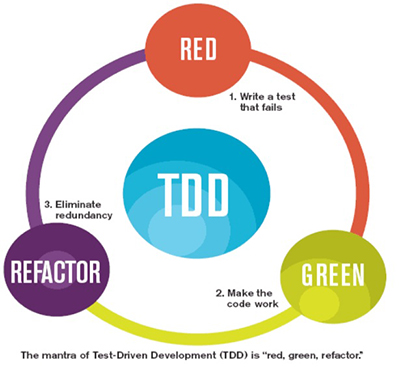
\includegraphics[scale=0.8]{img/TDD__logo.jpg}
    \caption{Esquema de práctica de programación de TDD (Test-Driven Deployment)\\ Fuente: \url{https://www.beeva.com/beeva-view/sistemas/cual-es-la-diferencia-entre-unit-testing-tdd-y-bdd/}}
    \label{fig:tdd}
\end{figure}
Seguir la práctica de programación TDD supone un cambio en la mentalidad de desarrollo, pensamos en qué queremos hacer con nuestro software y tras ello, cómo debe hacerlo. Adoptar esta metodología de trabajo es lenta, pero una vez adoptada el proceso de desarrollo es rápido y ágil. Afrontar el desarrollo mediante esta nueva práctica puede parecer un gasto de recursos debido al aprendizaje que supone adoptarla, pero esta es una inversión a largo plazo, ya que, ahorra recursos en el mantenimiento de nuestro código. Con TDD se garantiza una cobertura de código entre el 90\% y 100\%,lo que nos permite añadir funcionalidades de manera rápida y sencilla. Por último, esta forma de trabajo nos permite entender mejor el código y facilitar las contribuciones futuras en el software aumentando así la calidad del producto. 
\subsection*{Documentación}
Para un proyecto Python no solo se busca la legibilidad en el código, sino también en la documentación. A continuación se presentan unas buenas prácticas para facilitar tanto el uso como la contribución del proyecto. 
\subsubsection*{Documentación de  Proyecto}
Para cualquier proyecto de \emph{software} libre suele existir una documentación para usuarios y otra adicional para quien quiera contribuir al proyecto. Los siguientes ficheros que se comentan a continuación hacen referencia a esa documentación adicional y se centran en facilitar la contribución:\\
\begin{itemize}
    \item \textit{README}: Tal y como hemos mencionado, cuando creamos un repositorio GitHub es frecuente tener un fichero escrito en \emph{MarkDown} con el propósito de tener un breve resumen del contenido del proyecto o librería, la dirección del código principal. Este fichero es la entrada para cualquier usuario o contribuyente al proyecto. 
    \item \textit{INSTALL}: Este fichero es menos necesario en Python, ya que se reduce a ejecutar el comando \texttt{pip install [NAME\_MODULE]} o a ejecutar el script \emph{setup.py}. En él se añaden las instrucciones de instalación.
    \item \textit{LICENSE}: Fichero que todo proyecto debe contener en el que se especifica la licencia bajo la cual ponemos el proyecto disponible al usuario.
    \item \textit{TODO}: Este fichero es común incluirlo como sección en el fichero \emph{README}, su objetivo es listar los planes de desarrollo para el código.
    \item \textit{CHANGELOG}: Fichero que debe contener un resumen con los cambios producidos en el código respecto a la última versión.
\end{itemize}

\subsubsection*{Publicación del Proyecto}
Una vez que hemos tratado la documentación adicional que debemos incluir, la documentación principal deberá contener algunos o todos los siguientes componentes:
\begin{itemize}
    \item Una introducción con el propósito de mostrar de manera breve que podemos hacer con el proyecto.
    \item Un tutorial que debe enseñar los casos básicos detalladamente.
    \item Una referencia de la API, que suele generarse a partir del código mediante docstring\footnote{Un \emph{\textbf{docstring}} describe la operación de la función o clase, así como sus parámetros. Esta cadena de texto suele ir a continuación de la declaración de la función o en el fichero \textit{\_\_init\_\_.py} (marca un directorio como paquete) siguiendo unas reglas de escritura. }. 
    \item Documentación para el desarrollador donde se incluyen convenciones de código y la estrategia a seguir para el desarrollo de código. 
\end{itemize}

\subsection*{Escogiendo una licencia}
Al igual que para el software propietario o de autor, necesitamos escoger una licencia para nuestro proyecto. Una de las consecuencias de contribuir o usar un proyecto sin licencia es que es ilegal. Con ella otorgamos las cuatro libertades comentadas al inicio de este trabajo.Podemos distinguir los siguientes tipos como las principales licencias de código libre:
\begin{itemize}
    \item Licencias BSD: ejemplo de \textbf{licencia permisiva},centradas en dar una libertad total de distribución, modificación y uso del software. Permite que las versiones de los proyectos bajo esta licencia se distribuyan con otra distinta, incluida como software propietario.
    \item Licencias GPL: licencia que permite la libre distribución, modificación y uso, conservando los derechos de autor. Todo software que se desarrolle modificando el original y que contenga dicha licencia debe estar bajo está. Licencia considerada como primera licencia \textit{copyleft}.
    \item Licencias Apache: bajo este tipo de licencia se permite al usuario la distribución, modificación y distribuir alteraciones del software siempre y cuando que se mantenga el \emph{copyright}. Esta licencia no exige que se mantenga las versiones modificadas bajo la misma licencia, solo que se informe a los receptores de las modificaciones que bajo el código se ha utilizado dicha licencia Apache.
    \item Licencias Creative Commons: Estas licencias fueron creadas para la reutilización y compartición de cualquier material. Creative Commons que es la organización que creó dichas licencias, ofrece una manera de combinar derechos creando así seis posibilidades de licencias. El uso de estas licencias no es recomendable para \emph{software}.
    \begin{figure}[H]
        \centering
        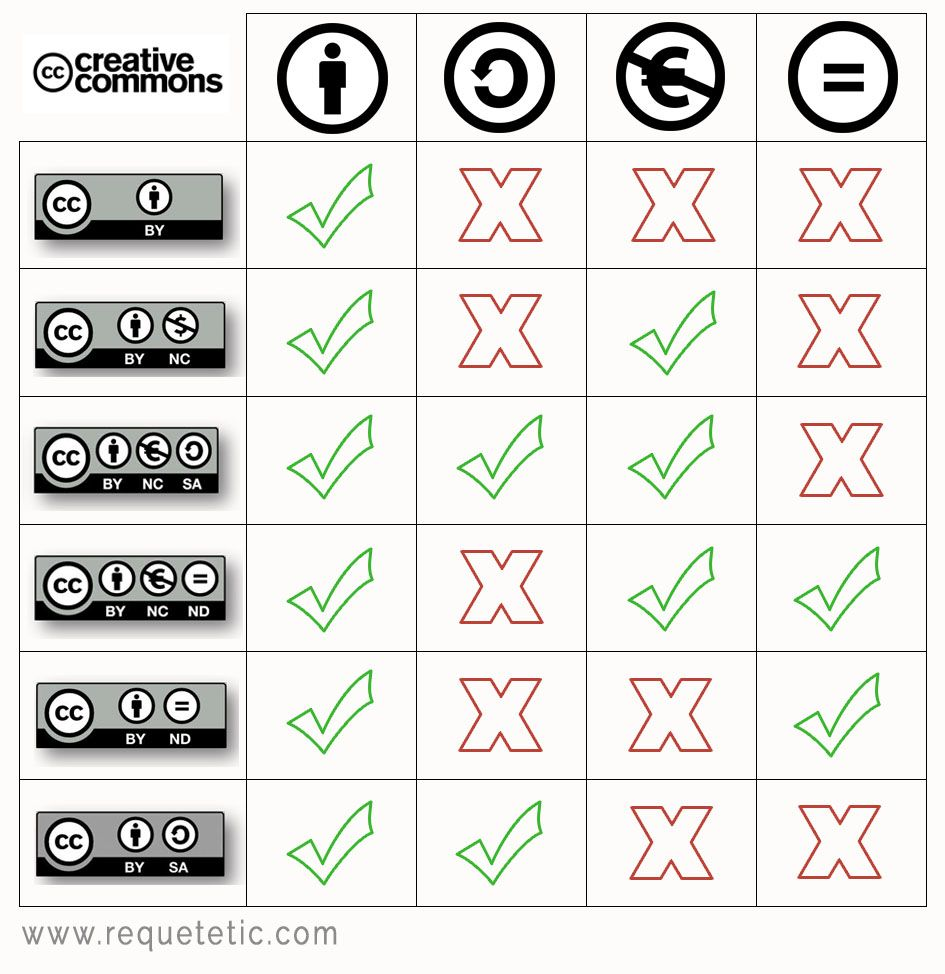
\includegraphics[scale=0.3]{img/licenciascondiciones.jpg}
        \caption{Licencias Creative Commons \\ Fuente: \url{http://www.requetetic.com/blog/licencias-creative-commons/}}
        \label{fig:licenses}
    \end{figure}
    
    Las diferentes licencias junto con los derechos que otorgan se puede comprobar en la figura \ref{fig:licenses}. Por ejemplo, si escogiéramos para una foto que hemos subido a Internet la segunda licencia, nos indica que podemos hacer uso de ella siempre y cuando se mencione al autor y no se realice un uso comercial. Sin embargo, nos permite modificar la obra original y cambiar la licencia de la obra derivada. 
    
    \item Licencias AGPL: licencias que derivan de las licencias GPL añadiendo una novedad, esta novedad obliga a distribuir el software modificado bajo su libre distribución.
\end{itemize}

Para nuestro proyecto, se ha decidido lanzar el software bajo la licencia Apache versión 2.0. Para poder aplicar dicha licencia, se crea un archivo de texto plano en el directorio raíz del proyecto con nombre \texttt{LICENSE} donde incluiremos todas las condiciones que está licencia aplica. 

\section{Gestión de código}
\label{subsec:}
Tras tratar con una breve guía de buenas prácticas para desarrollar y contribuir en un proyecto en Python, en este apartado abordaremos algunos de los servicios de gestión de código comentados en el capítulo \ref{chap:Arqui}. Para cada servicio que comentaremos a continuación, se hará una breve guía de utilización particularizándolo para nuestro proyecto PyCardio.

\subsection*{Travis}
\label{subsubsec:Travis}
Para la parte de integración continua se usará en nuestro proyecto Travis, ya comentado en el capítulo \ref{chap:Arqui}. Antes de empezar a integrar Travis en nuestro proyecto debemos tener una cuenta en GitHub y permitir a Travis acceder a ella. El siguiente paso es añadir a la raíz de nuestro proyecto un fichero de configuración \texttt{.travis.yml}, en él, se informa a Travis que tiene que hacer, donde podemos especificar la versión de lenguaje que utilizamos, el lenguaje, donde se encuentra nuestras pruebas de código, y un gran abanico de opciones que pueden variar debido al lenguaje utilizado. \\

Como integración continua se conoce a una práctica de \emph{software} que consiste en que los desarrolladores que estarán enviando cambios de forma periódica al repositorio compartido, se ejecuten pruebas de unidad en los nuevos cambios para identificar cualquier error. Lo que permite que tengamos siempre (tras cada cambio introducido) un \emph{software} libre de errores para probarlo antes de la fase de producción. \\

\begin{figure}[h]
\centering
\framebox[\textwidth]{%
\begin{minipage}{0.9\textwidth}
  \dirtree{%
.1 /PyCardio. 
.2 docs.
.2 PyCardio.
.3 HRV.
.3 ECG. 
.3 HRT.
.3 ReadHolter.
.3 \_\_init\_\_.py.
.2 .travis.yml.
.2 README.md.
.2 LICENSE.md.
.2 requirements.txt.
.2 setup.py.
}
\end{minipage}
}
\caption{Sistema de archivos PyCardio}
\label{fig:travisDir}
\end{figure}
El contenido del fichero \texttt{.travis.yml} para nuestro proyecto es el dado por la extracción de código \ref{travisPyCardio}. 
\begin{lstlisting}[caption={\texttt{.travis.yml} de PyCardio},label=travisPyCardio]
language: python
python:
  - "2.7"
install:
  - pip install -r requirements.txt
\end{lstlisting}
Observando el contenido del fichero, podemos diferenciar tres opciones:
\begin{itemize}
    \item \textbf{Language}: En esta opción indicamos a Travis el lenguaje del proyecto.
    \item \textbf{Python}: En este apartado indicamos todas las versiones de Python en la que queremos que se pruebe el proyecto. Para ello Travis creará un entorno virtual por cada versión que le indiquemos en él.
    \item \textbf{Install}: Con la orden install indicamos los comandos a ejecutar antes de probar, montar o construir el proyecto. En este caso con estos comandos instalaremos las dependencias de nuestro proyecto para el entorno virtual que crea Travis para cada versión. Estas dependencias vienen indicadas mediante el archivo \textit{requirements.txt}. 
\end{itemize}
Una de las opciones que no están incluidas en nuestro fichero \texttt{.travis.yml} es la orden \texttt{script}. En ella, se indica el fichero donde Travis puede encontrar los tests, y mediante que comando queremos que estos se ejecuten. Al no tener dichos tests implementados, no podemos incluir dicha orden en nuestro fichero. Aparte de la opción comentada, Travis tiene un abanico amplio para poder construir el proyecto de la manera más adecuada.

\subsection*{CodeCov}
\label{subsubsec:CodeCov}
Para apoyar la integración continua de nuestro proyecto, usaremos CodeCov. Nos aportará una medida de la cobertura que tenemos de pruebas de código sobre nuestro proyecto. \\
Para integrarlo en nuestro proyecto basta con conectarse a dicho servicio mediante GitHub, y modificar nuestro fichero \texttt{.travis.yml} quedando así como el de la figura \ref{travisCodecov}

\begin{lstlisting}[caption={\texttt{.travis.yml} para integrar CodeCov},label=travisCodecov]
language: python
python:
  - "2.7"
install:
  - pip install -r requirements.txt
  - pip install coverage
script: coverage run tests.py
after_success:
    - codecov
\end{lstlisting}

Al usar Travis para la integración continua, basta con añadir en el archivo  \textit{travis.yml} que tras la ejecución de las pruebas de código (mediante el comando \texttt{coverage run tests.py}) se ejecute el comando \texttt{codecov} donde se enviará el informe de cobertura a CodeCov. 

\subsection*{Read The Docs}
\label{subusub:rtd}
Como ya hemos comentado en el capítulo \ref{chap:Arqui} Read The Docs simplifica y automatiza la documentación de un proyecto desarrollado en Python. La documentación la cual Read The Docs usa para su servicio es la generada por dos herramientas MkDocs o Sphinx. Para PyCardio se ha hecho uso de la herramienta Sphinx. \\
¿Cómo trabaja Sphinx? La documentación que esta herramienta genera, lo hace a partir de documentos con lenguaje de marcado \textit{restructuredtext}. Estos ficheros los convierte en formato web (HTML), PDF o epub. \\


En nuestro caso, en vez de escribir la documentación de las funcionalidades de dichos módulos directamente en los documentos con el lenguaje de marcado mencionado ,usaremos la función \texttt{autodoc} de Sphinx, donde se generará documentación a partir de los \textit{docstrings} contenidos en el código, pero ¿qué es un \textit{docstring} de una clase, módulo o función?. Una de las prácticas que se debe llevar a cabo para un proyecto es la de tener correctamente detallada y documentada la funcionalidad de este. Para un proyecto Python usualmente se usa \textit{docstring}, que no es más que una cadena de texto que precede el código de una función, clase u objeto. Para nuestro ejemplo en la extracción de código \ref{docstring} observamos la documentación realizada al módulo \texttt{HRV.py} donde se muestra docstring del módulo, de la clase \texttt{HRV} y de la función \texttt{beat\_label\_filter}.

\begin{lstlisting}[language=python,caption=HRV.py,label=docstring]
""" 
 HRV.py 
 ====================================================================
 docstring of a HRV module
 Calculates from the RR intervals the statistical time domain variables and the geometrical variables to characterize the heart rate variability (HRV).The RR intervals used are all of them previous to valid tachograms according to the conditions evaluated in the characterization of the heart rate turbulence (HRT). 
 """
 class HRV(object):
    """ docstring of a HRV object """
    def beat_label_filter(self, beat_labels, numBeatsAfterV = 4):
        """
        docstring of a function of HRV class
        Function that identifies non-normal beats, and filters the rr signal to produce a vector identifying the positions where are non-normal beats.

        Input arguments:
            numBeatsAfterV <= 4
        Output arguments:
            ind_not_N:  has 1 in the position where there is a non-sinusal beat as classified by the label information.
        """
\end{lstlisting}

Una vez que tenemos nuestra implementación documentada tal y como se muestra con \textit{docstrings} necesitamos indicar en un documento \textit{restructuredtext} las funciones de las cuales vamos a generar su documentación, ya que Sphinx solo procesará aquellos documentos con dicho lenguaje de marcado. En nuestro caso, vamos a mostrar un caso sencillo en el que para la página principal de la documentación se mostrará la breve descripción\footnote{Dicha descripción es la misma que contiene el README.md del proyecto} del paquete de PyCardio y un enlace a la documentación del módulo HRV del paquete, del cual es el único del que disponemos de su documentación. \\
Este \texttt{index.rst} (página principal de nuestra documentación) esta compuesto por el código \ref{index}
\begin{lstlisting}[caption=\texttt{index.rst},label=index]
Welcome to PyCardio's documentation!
====================================

Python module to perform Cardiac Signal Analysis, namely:
  * **ECG analysis**: QRS detection, RR-interval time series extraction, ECG complete delineation
  * **Heart Rate Variability analysis**: Complete analysis from RR-interval time series:
    * Preprocessing
    * Time Domain Analysis
    * Frequency Domain Analysis
    * Nonlinear Analysis
    * Time-Frequency analysis
  * **Heart Rate Turbulence** analysis
  * **Atrial Fibrillation** analysis: both in ECG and intracavitary electrograms.
  * **Ventricular Fibrillation** Analysis
  * **Arrhythmia** analysis on 24 holter


.. toctree::
   :maxdepth: 1
   :caption: Contents:

   HRV

\end{lstlisting}
En este código observamos aparte de contenido plano, unas directivas, que son funciones del lenguaje \textit{restructuredtext}. La utilizada en esta página principal es \texttt{toctree} donde se indica cuál va a ser el árbol de nuestra documentación, en nuestro ejemplo, indicamos que como máximo sera de un nivel con la opción \texttt{maxdepth} y que tenemos como contenido HRV. Con la opción \texttt{contents}  indicamos que tenemos un contenido y que este es HRV. Sphinx buscará un documento el cual sea de nombre HRV y de lenguaje \textit{restructuredtext}, es decir, \texttt{HRV.rst}, en el cual se incluirá la estructura o contenido para la sección HRV, en este caso, para la página HTML del módulo HRV. \\
El contenido de \texttt{HRV.rst} es el dado por el código \ref{hrv}, que como vemos hacemos uso de la opción \texttt{autodoc} de sphinx. Para ello, indicamos donde debe hacer el uso de dicha opción con la directiva \texttt{automodule}, indicando de que módulo generamos la documentación. \begin{lstlisting}[caption=\texttt{HRV.rst},label=hrv]
Module HRV
==================

.. automodule:: HRV.HRV
  :members:

\end{lstlisting}

Una vez que tenemos escrito el esqueleto de nuestra documentación, mediante la ejecución del Makefile que genera Sphinx obtenemos nuestra documentación sobre HTML.

\begin{figure}[H]
    \centering
    \subfloat[Página Principal]{
        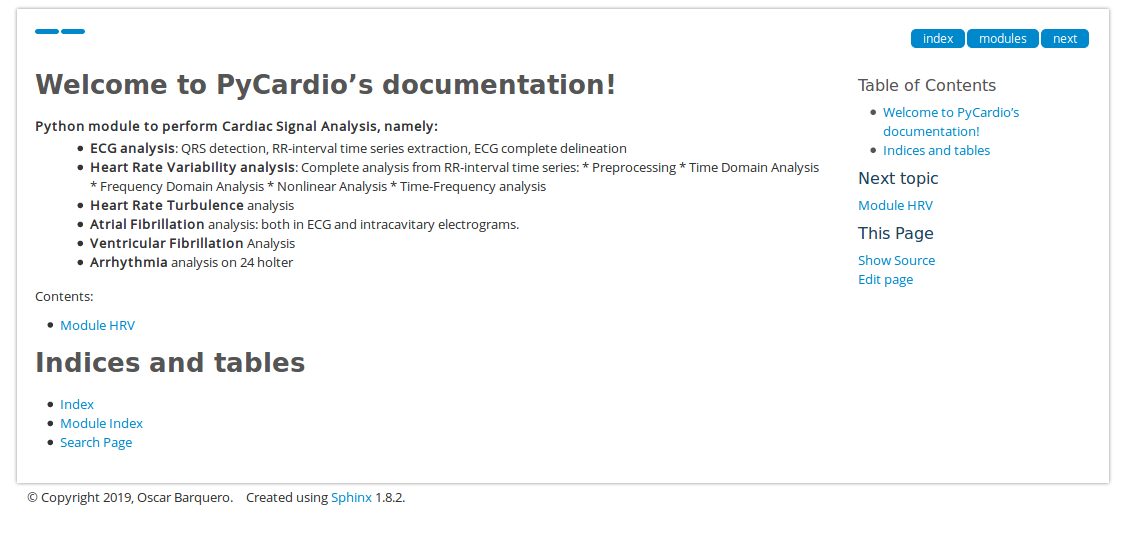
\includegraphics[scale=0.3]{img/sphinx_1.png}}
    \\
    \subfloat[Módulo HRV]{
        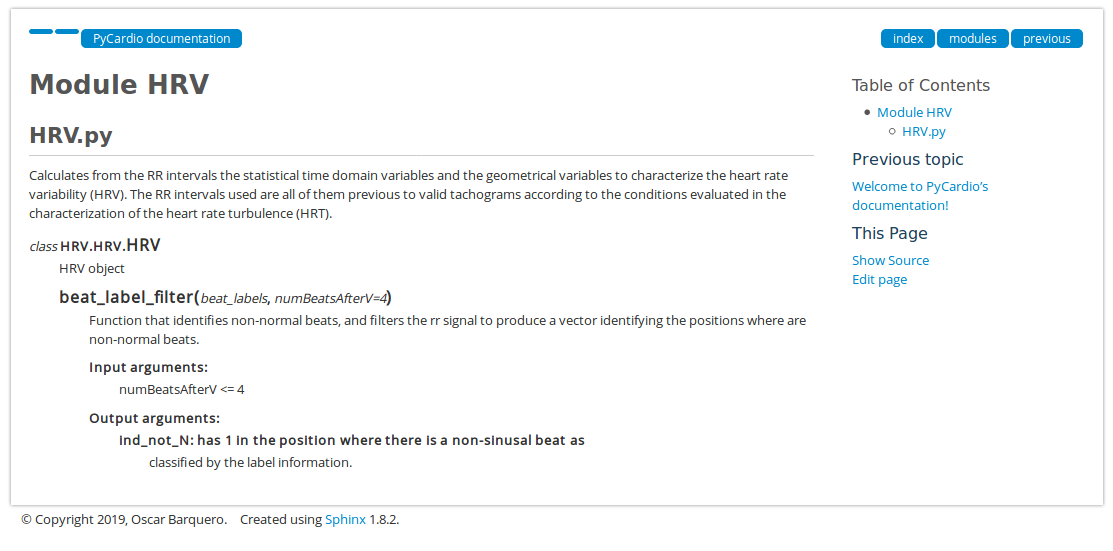
\includegraphics[scale=0.3]{img/sphinx_2.png}}
    \caption{Documentación generada por Sphinx}
    \label{fig:sphinx}
\end{figure}

Ya tenemos generada nuestra documentación, ahora podemos integrar esta con Read the docs, importando el repositorio donde se encuentre nuestro proyecto. Para ello Read The Docs localizará el archivo \texttt{conf.py} y generará la documentación y esta la alojará en su servidor. 


\subsection*{Empaquetado y Distribución}

El último aspecto que debemos considerar en gestión de código siendo este uno de los más importantes, es la de empaquetado y distribución. Una vez que el desarrollo se da por finalizado, y el equipo esta dispuesto a lanzar una primera producción del desarrollo de software necesitamos empaquetar el software diseñado para hacer de nuestro producto fácil de instalar para los usuarios y para nosotros, distribuirla. 


Tal y como se presentó en el capítulo \ref{chap:Arqui}, usaremos el repositorio oficial de aplicaciones de terceros,\emph{PyPI}, y el entorno de distribución Anaconda. Mostraremos así, el proceso para empaquetar \emph{pyCardio} para su posterior subida a \emph{PyPI}, y partiendo de esta, el empaquetado para Anaconda.

\subsubsection*{PyPI}
En Python existen dos módulos para el objetivo de empaquetar código, \textit{distutils} y \textit{setuptools}. Por lo comentado en el capítulo \ref{chap:Arqui} se hará uso de \textit{setuptools}, al extenderse de \textit{distutils} y poseer más funcionalidades. Antes de comenzar el empaquetado debemos estructurar nuestros ficheros y directorios correctamente. Tomando como ejemplo la estructura mencionada en la figura \ref{fig:dirPyPi}, y añadiendo los archivos necesarios de los servicios para integrarlos en nuestro proyecto que se han ido mencionado a lo largo de este capítulo, la estructura de \emph{pyCardio} es la expuesta en la figura \ref{fig:pyCardioDir}. \\

\begin{figure}[h]
\centering
\framebox[\textwidth]{%
\begin{minipage}{0.9\textwidth}
  \dirtree{%
.1 /PyCardio. 
.2 docs.
.2 PyCardio.
.3 HRV.
.3 ECG. 
.3 HRT.
.3 ReadHolter.
.3 \_\_init\_\_.py.
.2 .travis.yml.
.2 README.md.
.2 LICENSE.md.
.2 requirements.txt.
.2 setup.py.
.2 Makefile.
.2 tests.py.  
}
\end{minipage}
}
\caption{Estructura final PyCardio}
\label{fig:pyCardioDir}
\end{figure}

Como podemos observar los ficheros que componen nuestro proyecto, han sido ya comentados en las demás secciones de esta memoria describiendo su funcionalidad. Una vez que tenemos la estructura de ficheros y directorios correctamente, nos centramos en el archivo \textit{setup.py}, script de configuración. En él se hará uso de la función \textit{setup} incluida en el módulo \textit{setuptools}. Esta función puede tomar una amplia gama de parámetros. Para \emph{PyCardio}, usaremos las siguientes:
\begin{itemize}
    \item \textbf{name: } Nombre del paquete.
    \item \textbf{version: } Número de versión del paquete.
    \item \textbf{author: } Autor de la aplicación.
    \item \textbf{author\_email: } Dirección de correo del autor de la aplicación.
    \item \textbf{install\_requires: } Lista de las dependencias del paquete.
    \item \textbf{description: } Breve explicación del proyecto.
    \item \textbf{long\_description: } Descripción extensa del proyecto. De manera usual, coincide con el contenido de README.md
    \item \textbf{long\_description\_content\_type: } Tipo de lenguaje en el que esta escrito la descripción larga del proyecto.
    \item \textbf{url: } Dirección web donde se aloja el código del proyecto.
    \item \textbf{packages: } Lista de paquetes escritos en Python que se incluyen en la instalación de nuestro paquete. Para poder identificar cuales se incluyen se utiliza la función del módulo de \textit{setuptools},\textit{find\_packages()}.
    \item \textbf{classifiers: } Listado de las categorías a las que pertenece nuestro proyecto. Dichas categorías sirven para poder encontrar el paquete desarrollado en PyPI dependiendo del interés del usuario.
\end{itemize}

\begin{lstlisting}[language=python,caption=\textit{setup.py de pyCardio}]
import setuptools

setuptools.setup(
    name="PyCardioTest",
    version="0.0.6",
    author="Oscar Barquero",
    author_email="oscar.barquero@urjc.es",
    install_requires= [
        'numpy',
        'scipy',
        'matplotlib'
    ],
    description="Package for heart analysis",
    long_description=long_description,
    long_description_content_type="text/markdown",
    url="https://github.com/javierfm27/PyCardio",
    packages=setuptools.find_packages(),
    classifiers= [
        "Programming Language :: Python :: 3 ",
        "Natural Language :: English",
        "License :: OSI Approved :: Apache Software License",
        "Topic :: Scientific/Engineering :: Medical Science Apps.",
    ]
)

\end{lstlisting}

Una vez que tenemos nuestro script de configuración para \textit{setuptools}, para poder subir el proyecto a PyPI necesitamos crear un paquete de distribución. Para poder crear una fuente de distribución basta con ejecutar: \\
\texttt{python3 setup.py sdist}. \\
Esta fuente de distribución contiene una fase donde se crean los metadatos del paquete que como vemos en el comando ejecutado, se recogen a partir de \texttt{setup.py}. Cuando se genera la distribución  se crean dos carpetas, una que contendrá la información del paquete contenido en archivos planos de texto y otra carpeta "dist" donde se encontrará el archivo comprimido con el código del paquete que se ha desarrollado. \\

Para finalmente subir dicho proyecto a PyPI \footnote{El paquete que vamos a subir a PyPI, se subirá  a \url{https://test.pypi.org/}, ya que para que el proyecto pueda pertenecer a PyPI se necesita una aprobación de dicha subida.} usaremos el módulo \texttt{twine} porque la subida mediante el script \texttt{setup.py} basa la subida en archivos de texto plano poniendo en riesgo la cuenta y contraseña de PyPI. Por tanto, para subir dicho paquete a TestPyPI: \\
\texttt{twine upload dist/*}

\begin{figure}[H]
    \centering
    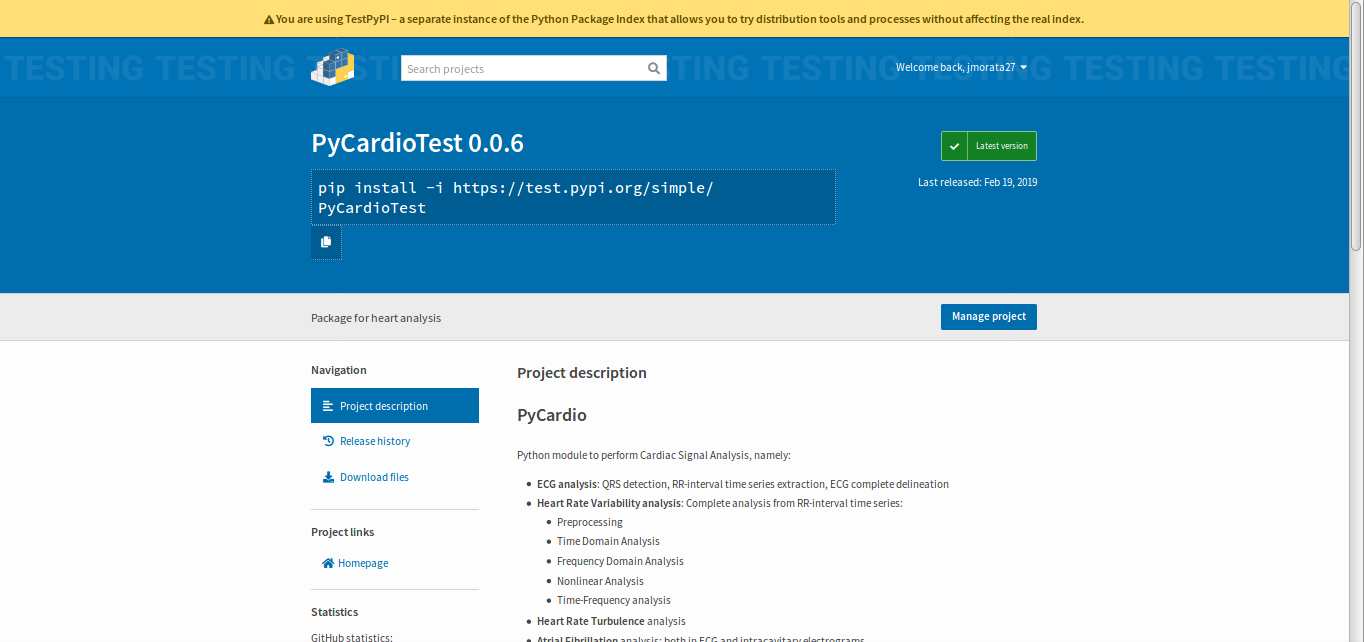
\includegraphics[scale=0.3]{img/testPyPi.png}
    \caption{pyCardio subido a Test PyPI}
    \label{fig:testPypi}
\end{figure}

\subsubsection*{Anaconda}
Conda

Para la creación del paquete conda partiremos del paquete que previamente hemos subido a TestPyPI. Conda para la creación de sus paquetes usa recetas, tal y como se introdujo en \ref{subsec:anaconda}. Para la creación de la receta de nuestro proyecto a partir de proyecto alojado en TestPyPI usaremos el módulo \texttt{conda-skeleton}, donde le pasaremos como argumento a la orden conda, la dirección del servidor TestPyPI y el nombre que tiene nuestro proyecto: \\
\texttt{conda-skeleton pypi PyCardioTest --pypi-url https://test.pypi.org/pypi/} \\
Esto creará una carpeta en nuestro directorio, este directorio es la mencionada receta que contendrá el fichero \texttt{meta.yaml} con los metadatos del paquete. Para generar el paquete el cual podrá ser distribuido mediante los canales de Anaconda, usamos \texttt{conda-build}. Al frente de generarlo, cuando ejecutamos: \\
\texttt{conda-build pycardiotest}\footnote{Siendo \textit{pycardiotest} el directorio de la receta generada con \texttt{conda-skeleton}} \\
Este comando sigue los siguientes pasos para construir el paquete:
\begin{enumerate}
    \item Lectura de metadatos de la receta generada
    \item Descarga del código fuente y lo almacena en una caché
    \item Organiza el código en un directorio de proyecto
    \item Aplicación de parches
    \item Creación de un entorno de construcción donde instala las dependencias necesarias para el paquete
    \item Ejecución del script \texttt{build.sh}
    \item Creación del paquete conda conteniendo todos los ficheros nuevos necesarios para el entorno de construcción junto con los metadatos para el paquete conda
\end{enumerate}
Así obtendremos el paquete conda, donde \texttt{conda build} se encarga de almacenarlo en el repositorio local de conda (o comúnmente denominado canal). En dicho repositorio local, además de encontrarnos con el paquete listo para su distribución o subida a un canal, contiene subdirectorios según la plataforma para la cuál se ha desarrollado el paquete, en estos subdirectorios nos encontraremos una lista de paquetes disponibles o un índice de repositorios. En nuestro caso el subdirectorio que se ha creado dando como único paquete disponible \texttt{PyCardioTest} es \texttt{linux-64}. Por cada subdirectorio se crea además de los paquetes conda, un archivo JSON \footnote{JSON es un formato de texto sencillo para intercambio de datos} listando todos los paquetes conda por subdirectorio recogiendo todos los metadatos del paquete. Así los paquetes disponibles en nuestro repositorio local son los mostrados por la figura \ref{fig:condaChannelLocal}. 

\begin{figure}[H]
    \centering
    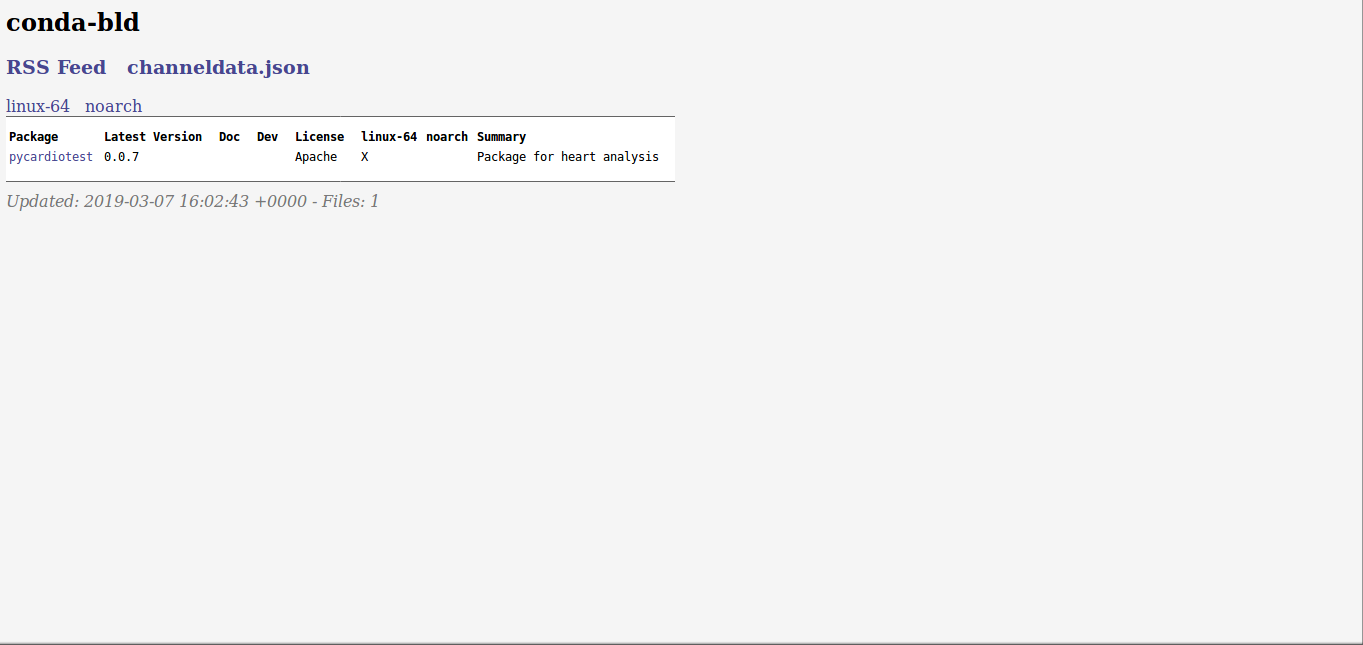
\includegraphics[scale=0.35]{img/condaLocalChannel.png}
    \caption{Repositorio local de paquetes conda disponibles}
    \label{fig:condaChannelLocal}
\end{figure}
